%%%%%%%%%%%%%%%%%%%%%%%%%%%%%%%%%%%%%%%%%
%
% (c) 2019 by Jennifer Laaser
%
% This work is licensed under the Creative Commons Attribution-NonCommercial-ShareAlike 4.0 International License. To view a copy of this license, visit http://creativecommons.org/licenses/by-nc-sa/4.0/ or send a letter to Creative Commons, PO Box 1866, Mountain View, CA 94042, USA.
%
% The current source for these materials is accessible on Github: https://github.com/jlaaser/pogil-polymers
%
%%%%%%%%%%%%%%%%%%%%%%%%%%%%%%%%%%%%%%%%%

\renewcommand{\figpath}{content/polymphys/mechanical-properties/viscoelasticity/figs}

\begin{activity}[Viscoelasticity of Polymeric Materials]

\begin{instructornotes}

	This activity introduces students to ...
	
	After completing this activity, students will be able to:
			\begin{enumerate}
				\item ...
			\end{enumerate}
	
			
	\subsection*{Activity summary:}
	\begin{itemize}
		\item \textbf{Activity type:} Learning Cycle
		\item \textbf{Content goals:} ...
		\item \textbf{Process goals:} %https://pogil.org/uploads/attachments/cj54b5yts006cklx4hh758htf-process-skills-official-pogil-list-2015-original.pdf
			written communication, critical thinking, information processing
		\item \textbf{Duration:} TBD %approx. 45 minutes without class discussion
		\item \textbf{Instructor preparation required:} 
			\begin{itemize}
				\item Prepare small samples of silly putty (or comparable silicone putty) for each student group
			\end{itemize}
		\item \textbf{Related textbook chapters:}
			\begin{itemize}
				\item \emph{Polymer Chemistry} (Hiemenz \& Lodge): ...
			\end{itemize}
	\end{itemize}

\end{instructornotes}

	%\textbf{Focus question:} Put a central question for the students to consider through this exercise here.

\begin{model}[Properties of Silicone Putty]
\label{model:sillyputty}

	Obtain a small sample of silicone putty from your instructor.
	
	Do the following experiments, and note your observations about how the material responds:
	
	\begin{itemize}
		\item Place a small ball of putty on a table, and hit it sharply with your hand.
			\begin{itemize}
				\item Observations:
				
				\vspace{1in}
			\end{itemize}
		
		\item Place a small ball of putty on your desk, and let it sit without touching it for 1-2 minutes.
			\begin{itemize}
				\item Observations:
				
				\vspace{1in}
			\end{itemize}
		
		\item Take a small piece of putty and stretch it between your hands.  Vary the rate at which you stretch it (quickly vs. slowly).
			\begin{itemize}
				\item Observations:
				
				\vspace{1.25in}
			\end{itemize}
		
	\end{itemize}

\end{model}


\begin{ctqs}

	\question In which of your experiments would you say the putty behaved more like a solid?  Briefly explain your reasoning.
	
		\begin{solution}[1in]
		\end{solution}
	
	\question In which of your experiments would you say the putty behaved more like a liquid?  Briefly explain your reasoning.
	
		\begin{solution}[1in]
		\end{solution}
	
	\question How did your observation of solid-like or liquid-like properties depend on how quickly you deformed or manipulated the putty?
	
		\begin{solution}[1in]
		\end{solution}
		
\end{ctqs}

\begin{infobox}

	Solid-like materials are typically described in terms of their \emph{modulus}, G.  For an elastic solid subjected to a strain (deformation) of size $\gamma$, the resulting stress (force), $\sigma$, is given by
	\begin{equation*}
		\sigma = G\gamma
	\end{equation*}
	
	Liquid-like materials are typically described in terms of their \emph{viscosity}, $\eta$.  For a liquid subjected to a strain $\gamma$, the resulting stress is 
	\begin{equation*}
		\sigma = \eta \frac{d\gamma}{dt} = \eta \dot\gamma
	\end{equation*}

\end{infobox}

\begin{ctqs}
		
		\question In which of your experiments on the silicone putty was the strain rate, $d\gamma/dt$, ...
			\begin{enumerate}
				\item ... large?
	
					\begin{solution}[1in]
					\end{solution}
				
				\item ... small?
			
					\begin{solution}[1in]
					\end{solution}
			\end{enumerate}
		
		\question Explain, in two or three complete sentences, how the properties you observed were related to the strain rate.
	
			\begin{solution}[1.5in]
			\end{solution}
		
		\question Explain, in one or two complete sentences, why you think we might describe this putty as a ``viscoelastic'' material.
	
			\begin{solution}[1.5in]
			\end{solution}
	
		
\end{ctqs}
	

\begin{model}[The Maxwell Model]

	One of the simplest models we can use to describe viscoelasticity of polymeric materials is the \emph{Maxwell model}.
	
	In this model, we imagine the response of the material as being represented by a spring and ``dashpot'' connected in series:
	
	\centerline{
\includegraphics[width=0.5\textwidth]{\figpath/model2-maxwellelement}}
	
	The spring ($\sigma = G_0\gamma$) reflects the elastic component of the response, while the dashpot ($\sigma = \eta_0\dot\gamma$) reflects the viscous component of the response.

\end{model}

\begin{ctqs}
		\question Start by considering \emph{only} the spring:
		
			\begin{enumerate}
				\item If I pull downward to extend the spring, hold onto it for some time, and then release it again, what do you expect to happen?  Briefly describe your prediction in 1-2 complete sentences.
	
					\begin{solution}[1.5in]
					\end{solution}
				
				\item The strain profile for the experiment described in this question is shown below:
				
					\centerline{\includegraphics[width=0.5\textwidth]{\figpath/model2-stepstrains}}
				
					On the following axes, sketch the stress that you would expect to measure over the course of this experiment.
				
					\centerline{\includegraphics[width=0.5\textwidth]{\figpath/model2-stressresponse}}
				
				\item Why might we say that the spring ``stores'' energy? sentences.
	
					\begin{solution}[1.5in]
					\end{solution}
			\end{enumerate}
			
		
		\question Next, consider \emph{only} the dashpot:
		
			\begin{enumerate}
				\item If I pull downward on the bottom of the dashpot, hold on for some time, and then release it again, what do you expect to happen?  Briefly describe your prediction in 1-2 complete sentences.
	
					\begin{solution}[1.5in]
					\end{solution}
				
				\item The strain profile for this experiment is the same as in the preceding question.  On the following axes, sketch the stress that you would expect to measure over the course of this experiment.
				
					\centerline{\includegraphics[width=0.5\textwidth]{\figpath/model2-stressresponse}}
				
				\item Why might we say that the dashpot ``dissipates'' energy?
	
					\begin{solution}[1.5in]
					\end{solution}
			\end{enumerate}
			
		\question Finally, consider the entire Maxwell element, with the spring and dashpot in series:
		
			\begin{enumerate}
				\item If I pull downward on the bottom of the Maxwell element, hold onto it for some time, and then release it again, what do you expect to happen?
	
					\begin{solution}[1.5in]
					\end{solution}
				
				\item The strain profile for this experiment is the same as in the preceding questions.  On the following axes, sketch the stress that you would expect to measure over the course of this experiment.
				
					\centerline{\includegraphics[width=0.5\textwidth]{\figpath/model2-stressresponse}}
			\end{enumerate}
			
\end{ctqs}
	
\vspace{-0.25in}
\begin{infobox}

	The experiments described in the preceding questions are \emph{step-strain} experiments, in which we quickly pull the material from its equilibrium position to a new position and hold it in place.  A step-strain experiment has the following strain profile:
	
	In a step-strain experiment, at times $t>0$, the total strain is constant, but how much of that strain is taken up by the spring and how much by the dashpot can change over time.
	The forces across the spring and dashpot, on the other hand, must be equal.
	Thus, at any point in the experiment,
	\begin{equation*}
		\gamma_0 = \gamma_{spring}(t) + \gamma_{dashpot}(t)
	\end{equation*}
	\begin{equation*}
		\sigma(t) = \sigma_{spring}(t) + \sigma_{dashpot}(t)
	\end{equation*}
	and 
	Because $\gamma_0$ is constant,
	\begin{align*}
		\frac{d\gamma_0}{dt} = 0 &= \frac{d\gamma_{spring}}{dt} + \frac{d\gamma_{dashpot}}{dt}\\
		&= \dot\gamma_{spring} + \dot\gamma_{dashpot}
	\end{align*}
	Substituting in $\gamma_{spring} = \sigma/G_0$ and $\dot \gamma_{dashpot} = \sigma/\eta_0$, we find
	\begin{equation*}
		0 = \frac{1}{G_0}\dot\sigma + \frac{1}{\eta_0}\sigma
	\end{equation*}
	Finally, solving this differential equation yields
	\begin{align*}
		\sigma(t) = \sigma_0 e^{-t G_0/\eta_0}  && \text{or} && \sigma(t) = \sigma_0 e^{-t /\tau}
	\end{align*}
	where $\tau = \eta_0/G_0$.

\end{infobox}
	
\begin{ctqs}
		\question As shown above, in a step-strain experiment, $\sigma$ decays exponentially with time.  Is this consistent with the qualitative prediction you made on the previous page?
	
					\begin{solution}[0.75in]
					\end{solution}
		
		\question At what time $t$ will $\sigma(t)$ drop to 1/e of its initial value?
	
					\begin{solution}[1.5in]
					\end{solution}
		
		\question Why might we refer to $\tau$ as the ``characteristic relaxation timescale''?  Explain your reasoning in 1-2 complete sentences.
	
					\begin{solution}[1.5in]
					\end{solution}
		
		\question For a highly crosslinked polymeric material, we expect $G_0$ to be large and $\eta_0$ to be small.
			\begin{enumerate}
				\item In this case, will $\tau$ be (relatively) large or small?  
	
					\begin{solution}[1in]
					\end{solution}
				\item In this case, will the stress $\sigma(t)$ decay (relatively) slowly, or quickly?
	
					\begin{solution}[1.25in]
					\end{solution}
				\item Is your prediction qualitatively consistent with your expectations for a mostly elastic solid?
	
					\begin{solution}[1in]
					\end{solution}
			\end{enumerate}
		
		\question For an un-crosslinked polymeric material above its glass transition temperature, we expect $G_0$ to be small and $\eta_0$ to be large.
			\begin{enumerate}
				\item In this case, will $\tau$ be large or small?  
	
					\begin{solution}[1.25in]
					\end{solution}
				\item In this case, will the stress $\sigma(t)$ decay (relatively) slowly, or quickly?
	
					\begin{solution}[1.25in]
					\end{solution}
				\item Is your prediction qualitatively consistent with your expectations for a mostly elastic solid?
	
					\begin{solution}[1.5in]
					\end{solution}
			\end{enumerate}
		
\end{ctqs}

\begin{model}[Small-Amplitude Oscillatory Shear Rheology]
\label{model:rheology}

	One of the most common experimental techniques used to characterize the viscoelasticity of polymeric materials is small-amplitude oscillatory shear rheology (SAOS).
	
	In a SAOS measurement, the sample is sandwiched between two surfaces that rotate back and forth at frequency $\omega$, resulting in a sinusoidally-varying strain:
	\begin{equation*}
		\gamma(t) = \gamma_0 \sin(\omega t)
	\end{equation*}
	
	The instrument (a rheometer) then measures the resulting force as a function of time, $\sigma(t)$, and breaks it down into two components: one that is proportional to $\sin(\omega t)$ and one that is proportional to $\cos(\omega t)$. The response of the material can thus be expressed as follows:
	\begin{equation*}
		G(t) = \frac{\sigma(t)}{\gamma_0} = G' \sin(\omega t) + G'' \cos(\omega t)
	\end{equation*}

\end{model}

%\vspace{0.25in}
\begin{ctqs}
		
		\question Which coefficient, $G'$ or $G''$, tells you how much of the response is directly proportional to the applied strain?
	
					\begin{solution}[1.1in]
					\end{solution}
		
		\question Does this coefficient tell you about the elastic response of the material, or the viscous response of the material?
	
					\begin{solution}[1.1in]
					\end{solution}
		
		\question For an applied strain $\gamma(t) = \gamma_0 \sin(\omega t)$, what is the strain \emph{rate}, $d\gamma/dt$?
	
					\begin{solution}[1.1in]
					\end{solution}
		
		\question Which coefficient, $G'$ or $G''$, tells you how much of the response is proportional to the strain rate?
	
					\begin{solution}[1.1in]
					\end{solution}
		
		\question Does this coefficient tell you about the elastic response of the material, or the viscous response of the material?
	
					\begin{solution}[1.1in]
					\end{solution}
		
		\question Remembering that elastic responses store energy, and viscous responses dissipate energy, explain why we call $G'$ the ``storage modulus'' and $G''$ the ``loss modulus'' of the material.
	
					\begin{solution}[2in]
					\end{solution}
			
\end{ctqs}

\begin{infobox}
	For the Maxwell model, the storage and loss moduli are given by:
	\begin{align*}
		G' = G_0 \frac{\omega^2 \tau^2}{\omega^2 \tau^2 + 1} && \text{and} && G'' = G_0 \frac{\omega \tau}{\omega^2 \tau^2 + 1}
	\end{align*}
	
	Plotting the moduli as a function of frequency yields plots that look something like the following:
				
		\centerline{\includegraphics[width=0.4\textwidth]{\figpath/model3-maxwellplot}}
	
	Note that both axes of this graph are plotted on a log scale, and the x axis has been scaled by the characteristic relaxation time, $\tau$.
	
\end{infobox}

\clearpage
\begin{ctqs}
	\question At low frequencies, which is greater, the storage modulus or the loss modulus?  Is this consistent with your expectations?
	
					\begin{solution}[1.1in]
					\end{solution}
	
	\question At high frequencies, which is greater, the storage modulus or the loss modulus?  Is this consistent with your expectations?
	
					\begin{solution}[1.1in]
					\end{solution}

	\question At what frequency is the storage modulus exactly equal to the loss modulus?  Give your answer in terms of the characteristic relaxation time, $\tau$.
	
		\emph{Note: you can answer this using either the graph or the equations, but you will probably find it easier to work from the equations.}
	
					\begin{solution}[1.75in]
					\end{solution}
	
	\question Rearrange your answer to the previous question to find an expression for the characteristic relaxation time in terms of the crossover frequency.
	
					\begin{solution}[1.25in]
					\end{solution}
	
	\question Using your answer to the previous question, find the characteristic relaxation time of the polymer characterized in the plot below:
				
		\centerline{\includegraphics[width=0.6\textwidth]{\figpath/model3-maxwellexample.jpg}}
	
					\begin{solution}[1.5in]
					\end{solution}
	
	\question If you were to pick up a sample of this polymer, would you expect it to feel more like a liquid or more like a solid?  Briefly justify your answer in 2-3 complete sentences.
	
		\emph{Hint: think about how the timescale on which you are observing/interacting with the polymer compares to the relaxation time!}
	
					\begin{solution}[2in]
					\end{solution}
	
\end{ctqs}
	

%\clearpage
\begin{exercises}

		\exercise Viscoelastic properties can arise from a number of molecular-scale interactions.  Which of the following do you think would give rise to viscoelastic properties in a polymeric material?  For each interaction that you think would cause a viscoelastic response, identify the physical process that you think would be most closely associated with the relaxation time of the material.
		
			\begin{enumerate}
				\item Covalent crosslinking of the polymer chains
				\item Hydrogen bonds (or other ``sticky'' noncovalent interactions) between polymer chains
				\item ``Tangling'' of long polymer chains around each other
			\end{enumerate}
			
		% exercise connecting to polymer processing? e.g. why is it important to control viscoelasticity in processing?
		
		\exercise In our discussion of the Maxwell Model, we considered a step-strain experiment, where we pulled the material to a set distance and then held it there.
		
			Another type of experiment we could conduct is a ``step-stress'' experiment, in which we simply begin pulling on the material with a constant force.  Make plots of (a) the applied stress and (b) the resulting strain that you would expect for this experiment.
		
		\exercise The Maxwell Model is one simple model that yields viscoelastic behavior.  Another model that gives viscoelastic behavior is the Voigt model, in which the spring and dashpot are connected in parallel rather than in series:
		
			\centerline{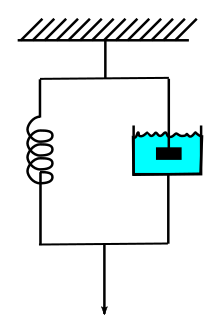
\includegraphics[width=0.25\textwidth]{\figpath/exercises-voigtelement}}
			
			In this case, the total \emph{stress} is the sum of the stresses across the two copmonents, while the total \emph{strain} is identical for each component.
			
			\begin{enumerate}
				\item Express the above statement using appropriate mathematical equations.  Then, find an expression for the total stress in terms of $G_0$, $\eta_0$, and $\gamma$.
				\item Qualitatively, how would you expect the Voigt element to respond to (a) a step strain experiment, and (b) a step stress experiment?  Plot the expected response for each case.
				\item Find a functional form for the strain, $\gamma(t)$, that results from a step stress of magnitude $\sigma_0$ (note: this is challenging, and requires some knowledge of differential equations).
					%Note: should coach this one more!
			\end{enumerate}
		
\end{exercises}
	
\end{activity}